\begin{figure}[h]
    \centering
    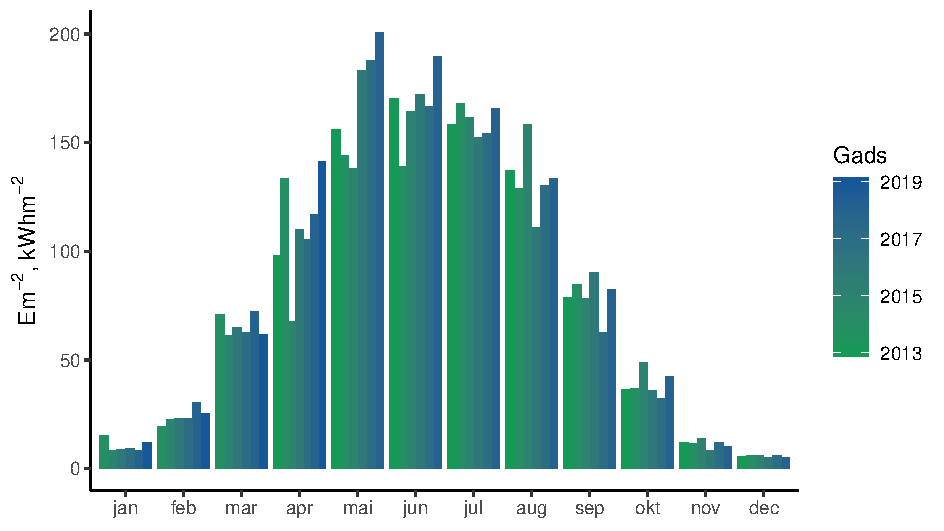
\includegraphics[width=\linewidth]{figures/meteo/statsYears.pdf}
    \caption{Solārā apstarojuma laika integrāļa atšķirības gada gaitā. LU Meteoroloģiskās stacijas dati 2013 -- 2019 periodā.}
    \label{fig:metYears}
\end{figure}
\begin{figure}[h]
    \centering
    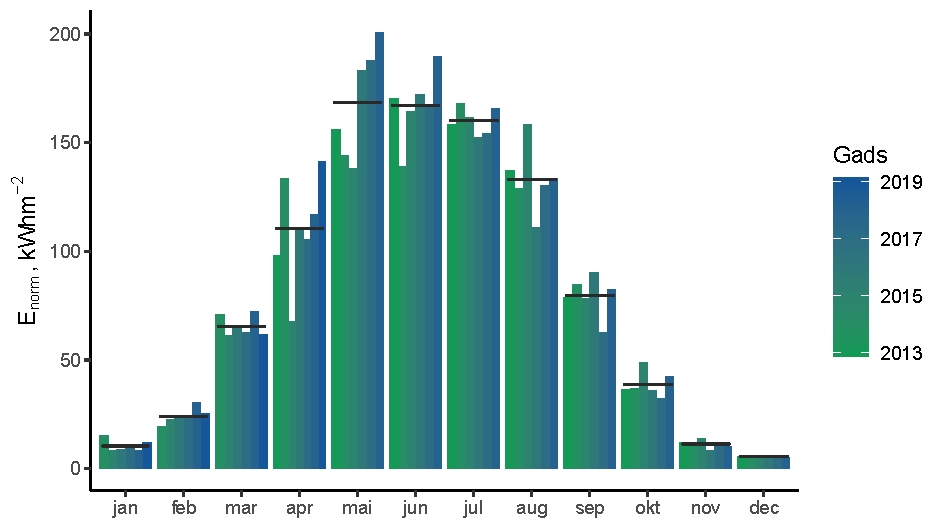
\includegraphics[width=\linewidth]{figures/meteo/meanYears.pdf}
    \caption{Solārā apstarojuma laika integrāļa atšķirības gada gaitā un to vidējās vērtības. LU Meteoroloģiskās stacijas dati 2013 -- 2019 periodā.}
    \label{fig:metYears_mean}
\end{figure}
\begin{figure}[h]
    \centering
    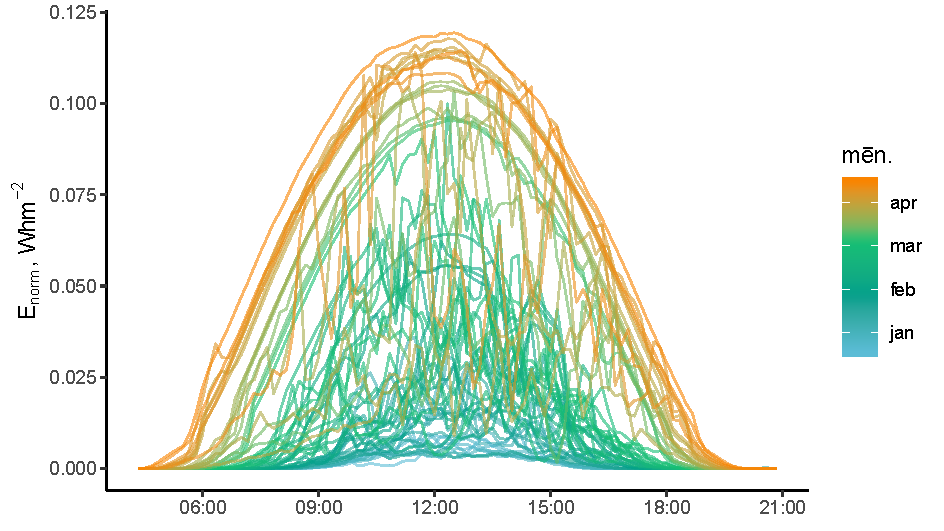
\includegraphics[width=\linewidth]{figures/meteo/sun19.pdf}
    \caption{Solārā apstarojuma izmaiņas dienas gaitā. LU Meteoroloģiskās stacijas dati 2019-01-01 -- 2019-04-31 periodā.}
    \label{fig:met_Irrad}
\end{figure}
\begin{figure}[h]
    \centering
    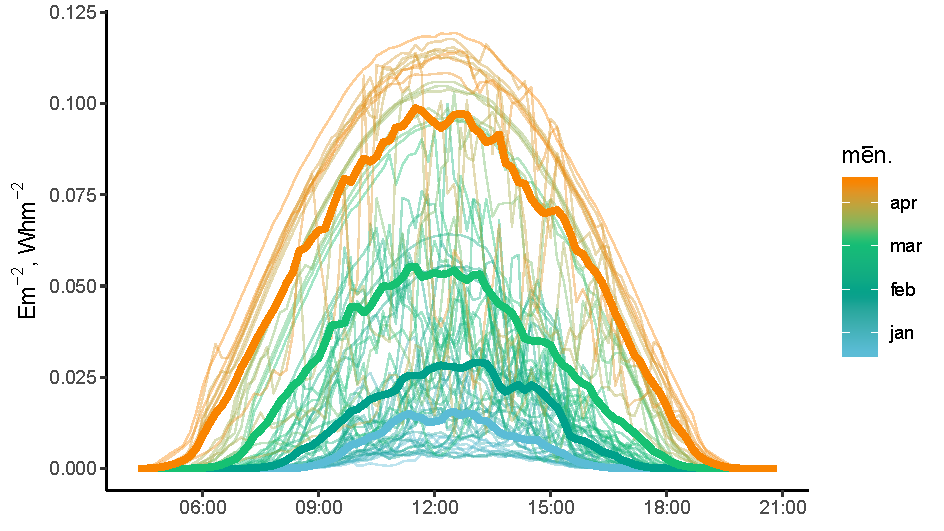
\includegraphics[width=\linewidth]{figures/meteo/mean19.pdf}
    \caption{Mēnesī vidējotas solārā apstarojuma izmaiņas dienas gaitā. LU Meteoroloģiskās stacijas dati 2019-01-01 -- 2019-04-31 periodā.}
    \label{fig:met_Irrad_mean}
\end{figure}
